\documentclass{../tudscript}
\begin{document}
   \sect{Orthogonalprojektion/ orthogonalzulegung}
        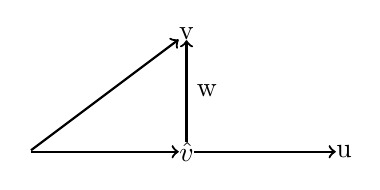
\begin{tikzpicture}
	        \node [inner sep=0pt] at (0, 0) (0) {};
	        \node [inner sep=0pt] at (4, 0) (u) {u};
	        \node [inner sep=0pt] at (2, 0) (vc) {$\hat{v}$};
	        \node [inner sep=0pt] at (2, 1.5) (v) {v};
	        
	        \draw [black, thick, ->] (0) -- (v);
	        \draw [black, thick, ->] (0) -- (vc);
	        \draw [black, thick, ->] (vc) -- (u);
	        \draw [black, thick, ->] (vc) -- node[right] {w} (v);
        \end{tikzpicture}\\

        \ilmath{v = \hat{v} + w \\
                \hat{v} = proj_u  v \\
                \hat{v} = proj_{span (\Set{u})}}
        $\hat{v}$ ist die \underline{Orthogonalprojektion von v auf u} und $ \bot u$
        bzw. $w \in U^\bot$.
        
        gegeben: $u, v$, gesucht: $\hat{v}, w$
        \ilmath{w = u - \hat{v}, \text{ falls } \hat{v} \text{ bekannt ist.}}

        gesucht: $\hat{v}$. Wir setzen voraus:
        
        \ilmath{\hat{v} = k \cdot u \text{ mit } k \in \bR}

        (denn $\hat{v} \in U = span \Set{u}$)
    
        \ilmath{v = \hat{v} - w = ku + w \implies v \circ u = (k \cdot u + w) \circ u = k (u \circ u) + \underbrace{w \circ u}_{ = 0} \\
                \implies v \circ u = k(u \circ u) \implies k = \frac{v \circ u}{u \circ u}}
        
        Zusammenfassung:
        \ilmath{\hat{v} = \frac{v \circ u}{u \circ u} \cdot u}

        \ssect{Beispiel}
        $v = \vect{2}{0}, u = \vect{1}{1}$ gesucht: $\hat{v} = proj_u (v), w \in span (\Set{u})hat\bot$ mit $v = \hat{v} + w$\\
        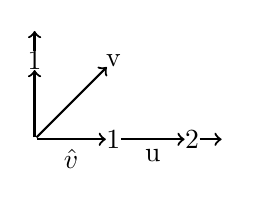
\begin{tikzpicture}
        \node [inner sep=0pt] at (0, 0) (0) {};
        \node [inner sep=0pt] at (2.4, 0) (x) {};
        \node [inner sep=0pt] at (0, 1.4) (y) {};
        \node [inner sep=0pt] at (0, 1) (y1) {1};
        \node [inner sep=0pt] at (1, 0) (x1) {1};
        \node [inner sep=0pt] at (2, 0) (x2) {2};
        \node [inner sep=0pt] at (1, 1) (z) {v};
        
        \draw [black, thick, ->] (0) -- (y1);
        \draw [black, thick, ->] (0) -- node[below] {$\hat{v}$} (x1);
        \draw [black, thick, ->] (x1) -- node[below] {u} (x2);
        \draw [black, thick, ->] (y1) -- (y);
        \draw [black, thick, ->] (x2) -- (x);
        \draw [black, thick, ->] (0) -- (z);
        \end{tikzpicture}\\

        \ilmath{\hat{v} = \frac{\vect{1}{1} \circ \vect{2}{0}}{\vect{2}{0} \circ \vect{2}{0}} \vect{2}{0} = \frac{2}{4} \vect{2}{0} = \vect{1}{0} \\
                w = v - \hat{v} = \vect{1}{1} - \vect{1}{0} = \vect{0}{1}}
    
    \sect{Satz: Orthogonalzerlegung}
        Sei V ein euklidischer $\bR$-VR, U ein U-VR von V, $v \in V$.
        
        Sei $\Set{u_1, u_2, \ldots, u_k}$ eine Orthogonalbasis von U.
        Dann existiert eine Darstellung: $v = \hat{v} + w$ mit $\hat{v} \in U, w \in U^\bot$,
        \ilmath{\hat{v} = \frac{v \circ u_1}{u_1 \circ u_1} u_1 + \frac{v \circ u_2}{u_2 \circ u_2} u_2 + \ldots + \frac{v \circ u_k}{u_k \circ u_k} u_k, w = v - \hat{v}}

        \ssect{Beweis}

        $\hat{v} \in U = span (\Set{u_1, \ldots, u_k})$
        zu zeigen: $w \in U^\bot$

        Sei $i \in \Set{1, \ldots, k}$:
        \ilmath{w \circ u_i &= (v - \hat{v}) \circ u_i \\ 
                            &= v \circ u_i - \hat{v} \circ u_i \\
                            &= v \circ u_i - \frac{v \circ u_1}{u_1 \circ u_1} u_1 \circ u_i - \ldots -\frac{v \circ u_i}{u_i \circ u_i} (u_i \circ_i) - \frac{v \circ u_k}{u_k \circ u_k} (u_k \circ u_i) \\
                            &= v \circ u_i - \frac{v \circ u_i}{u_i \circ u_i} (v \circ w) \\
                            &= v \circ u_i - v \circ u_i \\
                            &= 0}
    
    \sect{Gram-Schmidt Verfahren}
        Gram-Schmidt Verfahren zur Konstruktion von Orthogonalbasen.
        Gegeben: Basis $\Set{b_1, b_2, \ldots, b_k}$ eines k-dim UVR des eukl.
        $\bR$-VR V.
        
        Gesucht: Ortogonalbasis $\Set{u_1, \ldots, u_k}$ dieses UVR.
        d.h. 
        \ilmath{\forall i, j \in \Set{1, \ldots, k}: u_i \circ u_j =0}\\
        
        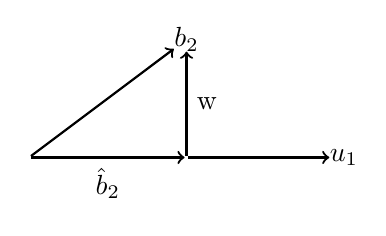
\begin{tikzpicture}
	        \node [inner sep=0pt] at (0, 0) (0) {};
	        \node [inner sep=0pt] at (4, 0) (u) {$u_1$};
	        \node [inner sep=0pt] at (2, 0) (vc) {};
	        \node [inner sep=0pt] at (2, 1.5) (v) {$b_2$};
	        
	        \draw [black, thick, ->] (0) -- (v);
	        \draw [black, thick, ->] (0) -- node[below] {$\hat{b}_2$} (vc);
	        \draw [black, thick, ->] (vc) -- (u);
	        \draw [black, thick, ->] (vc) -- node[right] {w} (v);
        \end{tikzpicture}\\
        
        \ilmath{u_1 &= b_1 \\
                u_2 &= b_2 - \frac{b_2 \circ u_1}{u_1 \circ u_1} u_1  \text{ dann gilt } u_1 \bot u_2 \\
                u_3 &= b_3 - \frac{b_3 \circ u_1}{u_1 \circ u_1} u_1 - \frac{b_3 \circ u_2}{u_2 \circ u_2} u_2 \text{ dann gilt } u_3 \bot u_1 \land u_3 \bot _2 \\
                \ldots}

        Zusammengefassung: \underline{Verfahren von Gram-Schmidt}:
        \ilmath{u_1 &:= b_1 \\
                u_{i + 1} &:= b_{i + 1} - proj_{span (\Set{u_1, \ldots u_i})}}
    \sect{Best Approximation}
        Sei V ein euklidischer $\bR$-VR, $v \in V$, U ein UVR von $\bR$, $\hat{v} = proj_{U} (v) \in U$
    
        Dann gilt:
        \ilmath{||v - \hat{v}|| \leq ||v - u || \text{ für alle } u \in U}

        \begin{tikzpicture}
	        \node [inner sep=0pt] at (0, 0) (0) {};
	        \node [inner sep=0pt] at (4, 0) (u) {u};
	        \node [inner sep=0pt] at (2, 1.5) (v) {v};
	        \node [inner sep=0pt] at (1.4, 0) (s1) {};
	        \node [inner sep=0pt] at (2, 0) (s2) {};
	        \node [inner sep=0pt] at (2.6, 0) (s3) {};
	        
	        \draw [black, thick, ->] (0) -- (v);
	        \draw [black, thick, ->] (0) -- node[below] {$\hat{v}$} (vc);
	        \draw [black, thick, ->] (vc) -- (u);
	        \draw [black, thick] (0) -- (u);
	        
	        \draw [black, thick, decorate, decoration=snake] (v) -- (s1);
	        \draw [black, thick, decorate, decoration=snake] (v) -- (s2);
	        \draw [black, thick, decorate, decoration=snake] (v) -- (s3);
        \end{tikzpicture}\\ 

        Sei $Ax = b$ ein LGS mit $\mathscr{L} = \emptyset$.
        (denn $b \notin \underbrace{Col (A)}_{ = U}$) 
        
        $b = \hat{b} + w$ mit $\hat{b} \in U, w \in U^\bot$
        
        $\hat{b} = proj_U (b)$

        Statt $Ax = b$ wir das LGS $Ax = \hat{b}$ gelöst. Lösung $\mathscr{L} = \hat{x}$
        ($Ax = \hat{b}$ ist lösbar wegen $\hat{b} \in U$)

        Die Lösung ist bestmöglich, weil $\hat{b}$ die Projektion von b auf U und der Satz
        über die Bestapproximation gilt, d.h.
        \ilmath{||b - \hat{b}|< \text{ minimal ist.}}

        \ssect{Beispiel}
        \ilmath{\begin{pmatrix} 4 & 0 \\ 0 & 2 \\ 1 & 1 \end{pmatrix} \vect{x}{y} = \vectt{2}{0}{11}}
        zuerst eine Orthogonalbasis von Col (A) berechenen (und GRAM-SCHMIDT), damit $proj_U (b) = \hat{b}$,
        dann $Ax = \hat{b}$

        Zu lösen ist (nur) das \underline{Normalgleichungssystem} $A^T A x = A^T b$
\end{document}
